\chapter{Ad Hoc tīkla teorētiskie aspekti}\label{sec:tris}

\section{Komunikācijas modeļi}
Tīklā notiekošie procesi var būt apskatīti kā fizikālie procesi vai arī kā protokolu norises darbība. Savā grāmatā Perkins piedāvā divus Protokolu un fizisku komunikācijas modeļus \cite{perkinsBook}. Protokola modelis (\textit{Protocol Model}) nosaka, ka mezgls $i$ veiksmīgi pārraida mezglam $j$, ja kaimiņ mezgls $X_{k}$ uzsākot pārraidi nepārraus savienojumu starp $X_{i}$ un $X_{j}$ mezgliem. Matemātiski to var izteikt sekojoši:
\begin{equation}
 \mid X_{k}-X_{j}\mid\geq(1+\Delta)\mid X_{i}-X_{j}\mid ,
\end{equation}
savienojums starp $X_{i}$ un $X_{j}$ mezgliem.
Fiziskais  modelis (\textit{Physical Model}) nosaka, ka mezgls $i$ veiksmīgi pārraida mezglam $j$, ja mezglā $j$ signāla un interferences attiecība (\acs{SIR}) ir
\begin{equation}
 SIR=\frac{\frac{P_{t}}{|X_{i} -X_{j}|^\alpha}}{N_{o}+\sum\limits_{k\neq i}\frac{P_{k}}{|X_{k}-X_{j}|^\alpha}}\geq\beta ,
\end{equation}
kur \gls{p_t} ir mezgla $i$ pārraides jauda, $\alpha$ ir pārraides trakta zudumu koeficients, $N_{o}$ ir trokšņa līmenis un $\beta$ ir minimālā nepieciešama signāla un interferences attiecība (\acs{SIR}) kas ir nepieciešams veiksmīgai datu pārraidei.  Gadījumā kad $\alpha >2$ un visi mezgli pārraida ar vienādu $P_{t}$, abu modeļu aprēķinu rezultātiem ir jābūt vienādiem \cite{perkinsBook}.


\section{Tīkla modeļi}
\subsection{Statiskais ekspromta tīkls}
Savā darbā P.Gupta un P.R.Kumar \cite{gupta} pēta statisko bezvadu tīklu caurlaidspēju. Tīkla modelis ir vienības sfēra kurā novietoti $n$ identiski mezgli. Skaitlis $n$ ir nemainīgs un mezgli izvietoti nejauši. Visi mezgli raida vienā kanālā un mezgli savstarpēji traucē izraisot interferenci. No avota līdz galamērķim paketes tiek pārraidītas pa daudzposmu maršrutu, izveidotie maršruti ir taisnas līnijas (iespējamais īsākais ceļš). Katrs mezgls var būt arī avots, galamērķis vai retranslējošs mezgls. Izmantojot Voronoi diagrammu ar sfēras virsmu $S^2$ (\seename ~\figurename.~\ref{fig:voronoi}), viņi pierādīja ka eksistē tāda Voronoi diagramma kas nodrošina:
\begin{itemize}
 \item Katra Voronoi šūna $V \in \nu_{n}$ iekļauj sevī disku ar laukumu $\frac{100\log{n}}{n}$ un
 $\rho(n)$ vienāds ar diska rādiusu ar laukumu $\frac{100\log{n}}{n}$ uz $S^2$ virsmas.\footnote{Šī diska laukums uz $S^2$ virsmas ir mazāk par $\pi \rho^2$}
\item Katra Voronoi sūna ir ietverta diskā ar rādiusu $2\rho(n)$
\end{itemize}

\begin{figure}[htb!]
\centering%

\includegraphics{./graph/voronoi}
\caption{$S^2$ virsmas Voronoi diagramma uz sfēras \cite{gupta}}
\label{fig:voronoi}
\end{figure}

Pārejot uz 2-dimensionālo plakni rādiuss būs $e(n) = c\sqrt{n\log(n)}$, ar konstanti $c$ lielāku par 0. Tīkla mezgli ir nejauši izvietoti līdz ar to visām Voronoi šūnām $V \in \nu_{n}$ ir iregulāra forma un katrā no šūnām ar $\zeta \geq 1-\frac{c}{n}$ varbūtību ir izvietots vismaz viens mezgls, kur $c$ lielums atbilst savienojuma prasībām \cite{gupta}. Izēveloties mezglu pārraides diapazonu $8e(n)$, tas ļauj nodrošināt komunikāciju ar kaimiņ-mezgliem kas atrodas $8e(n)$ attālumā. Divas šūnas izraisa savstarpējus traucējumus, ja viena no šūnām ir mezgla $(2+\Delta)8e(n)$ attālumā no jebkuras mezgla otras šūnas. $\Delta$ ir pozitīvs skaitlis, to pielieto modelējot situāciju, kad ir nepieciešamība nepiļaut blakus esošiem mezgliem pārraidīt vienlaicīgi vienā kanālā.

Izmantojot ''\textit{Protocol}'' un ''\textit{Physical}'' modeļus var pierādīt, ka statisko bezvadu ekspromta tīklu caurlaidspēja vienāda ar $\Theta({\frac{1}{\sqrt{n}}})$ gadījuma kad mezgli ir patvaļīgi novietoti tīkla laukumā. Un $\Theta(\frac{1}{\sqrt{n\log(n)}})$ ar nejauši izvietotiem mezgliem. Neņemot vērā to, kādā veidā ir izvietoti mezgli, caurlaidspēja samazinās pieaugot kopējam $n$ mezglu kaitam.


\subsection{Mobilais Ad Hoc tīkls ar viena-posma maršrutu}
Grossglauser un Tse \cite{grossglauser} pievādā izmantot viena-posma datu pārraides shēmu MANET. Šī shēma izmanto vienkāršo trakta izplatīšanas modeli, kurā datu avots izvēlas īsāko maršrutu (short-path) un rezervē to. Kaimiņmezgli tiek izvēlēti kā retranslējoši, ja tie ir tieši savienoti ar galamērķi (tikai viens posms). Tīkla modelis ir normalizēts vienības disks kura laukumā izvietoti $n$ mobilie mezgli. Lai atvieglotu analīzi, tiek pieņemts, ka informācijas apmaiņa notiek laika intervālos. Atrašanās vieta mezglā $i$ laika periodā $t$ apzīmēta ar $X_{i}(t)$. $\{X_{i}(\cdot)\}$ kas ir stacionārs un ergodisks process izkliedēts uz diska virsmas, kura mezgli kustas pēc neatkarīgi un viendabīgi izkliedētas (\acs{iid}) trajektorijas. Katrā no laika intervāliem, plānotājs izlemj kurš no mezgliem būs datu avots, retranslējošs mezgls vai galamērķis. Tādā veidā tiek panākts, ka pāris avots - galamērķis ir nemainīgs laika periodā.

Avotam $i$ ir ziņojums uz galamērķi $d(i)$ laika periodā $t$. Tā kā mezgliem $i$ un $d(i)$ savienojums ilgst vidēji $\frac{1}{n}$ laikā periodu, tad ziņojums būs piegādāts $d(i)$ $\frac{1}{n}$ vai $\frac{2}{n}$ maršrutā ar retranslējošo mezglu. Grossglauser un Tse pieņem ka katra pakete var būt pārsūtīta ne vairāk kā vienu reizi.

Saskaņā ar $Physical Model$ laika brīdī $t$ mezgls $j$ var saņemt informāciju no $i$ ar noteikto ātrumu $B$ [b/sec] , ja
\begin{equation}
SIR=\frac{P_{t}(t)g_{ij}(t)}{N_{0}+\frac{1}{M}\sum\limits_{k\neq
i}P_{k}(t)g_{ij}(t)}=\frac{P_{t}(t)g_{ij}(t)}{N_{0}+\frac{1}{M}I}\geq\beta,
\end{equation}
kur $P_{t}(t)$ ir mezgla $i$ pārraides jauda, $g_{ij}(t)$ - savienojuma garuma pieaugums no mezgla $i$ līdz $j$, $M$ - sistēmas apstrādes pieaugums un $I$ kopējā interference mezglā $j$. Savienojuma garuma pieaugums $g_{ij}(t)$ ir no attāluma atkarīga funkcija \cite{grossglauser},
\begin{equation}
 g_{ij}(t)=\frac{1}{|X_{i}(t)-X_{j}(t)|^\alpha}=\frac{1}{r_{ij}^\alpha(t)},
\end{equation}
kur $r_{ij}(t)$ ir attālums starp $i$ un $j$.

No iepriekš teiktā izriet, ka katrs no mezgliem nosūta datus divos etapos. Pirmajā etapā notiek pakešu pārraide no avota uz retranslācijas mezglu un otrajā no retranslācijas mezgla uz galamērķi. Abi posmi notiek paralēli, bet  2. etapam ir absolūta prioritāte visos ieplānotajos avots-galamērķis pāros. Tādēļ, ka mezglu trajektorija ir neatkarīga un viendabīgi izkliedēta un sistēma atrodas stabilā stāvoklī, ilgtermiņa caurlaidspēja starp jebkuriem diviem mezgliem ir vienāda ar varbūtību ka šie divi mezgli tiks izvēlēti kā iespējamie avots-galamērķis pāris. Saskaņā ar \cite{grossglauser} šī varbūtība ir vienāda ar $\Theta(\frac{1}{n})$. Nejauši izvēlētais avots-galamērķis pāris var tikt savienots tieši vai caur vienu retranslējošo mezglu. Tādējādi, pakalpojuma līmenis ir $\lambda_{j} = \Theta(\frac{1}{n})$ izmantojot retranslācijas mezglu vai tiešo savienojumu. No tā izriet, ka kopējā caurlaidspēja avots-galamērķis pārim $\lambda_{T}$ ir
\begin{equation}
 \lambda_{T}=\sum\limits_{j=1, j\neq i}^{n}\lambda_{j}=\sum\limits_{j=1, j\neq
i}^{n}\Theta
(\frac{1}{n})=\Theta\lgroup\frac{n-1}{n}\rgroup\xrightarrow{
n\rightarrow\infty} \Theta(1).
\end{equation}
Tātad šī shēma sasniedz $\Theta(1)$ caurlaidspēju avots-galamērķis pārī tad, kad $n$ mezglu skaits tiecas uz bezgalību. Tomēr tāda viena lēkuma pārraide izraisa lielu pakešu aizkavēšanos un attiecīgi ar $n$ pieaugumu tiecas uz bezgalību.

\subsection{Mobilais Ad Hoc tīkls ar daudzposmu maršrutu}\label{sec:moby}
O.Tonguz savā darba \cite{qoS_mobility} piedāvā jaunu veidu kā reprezentēt mobilā tīkla topoloģiju. Lai mazinātu malas efektu, tiek uzskatīts ka tīkla virsma ir apļa  forma. Šis pieņēmums palīdz vienkāršot aprēķinus, jo mezgliem kas izvietoti pie pašas tīkla robežas ir mazāks kaimiņ-mezglu skaits salīdzinājuma ar pārējiem mezgliem. Gadījumā, ja tīkla virsma ir apaļa virsma, tad visiem tīklā esošajiem mezgliem ir vienāds kaimiņu skaits  neatkarīgi no tā, vai tas atrodas uz tīkla malas vai centrā. Šeit ir svarīgi atzīmēt ka, dēļ šī pieņēmuma var rasties neliela atšķirība ar reālo sensoru tīklu.

\begin{figure}[ht!]
 \centering
\includegraphics[scale=0.6]{./graph/tier.png}
\caption{Mobilo mezglu novietošana tīklā}
\label{fig:topo}
\end{figure}

Lai iegūtu ieskatu šajā problēmā, tiek pieņemts, ka tīkls ir taisnstūra režģis ar mezgliem izvietotiem to krustojumos un katram mezglam ir četri tuvākie kaimiņi (\seename~\figurename.~\ref{fig:topo}). Sakarā ar kvadrāta režģveida struktūru attālums līdz tuvākajam kaimiņam  ir fiksēts lielums \gls{r_link}  un maršruts līdz jebkuram mezglam ir vienāds ar vienāda garuma posmu virkni. Konstruējot kvadrāta režģi no $N$ mezgliem uz apļa virsmas ar laukumu $A$ ir viens un tas pats kā $N$ mazie kvadrāti ar laukumu $r_{link}^{2}$ ievietot lielā kvadrātā  ar laukumu $A$. No kā izriet ka $Nr_{link}^{2} = A$ un līdz ar to attālums starp diviem tuvākiem kaimiņiem var tikt izteikts sekojoši \cite{qoS_mobility}:
\begin{equation}
r_{link}=\sqrt{\frac{A}{N}}=\frac{1}{\sqrt{\rho_{s}}}
\label{eq:rlink}
\end{equation}
Kur \gls{rho} ir mezglu telpiskais blīvums. Tātad, kāda laika perioda $t$ avotam $n_{A}$ ir ziņojums uz galamērķi $n_{G}$ (att.~\ref{fig:topo}). Maršruts no $n_{A}$ līdz $n_{G}$ izmanto 2 retranslējošus mezglus ($r_{1}$, $r_{2}$) un tā kopējais garums ir 3$r_{link}$. Līdz ar to attālums starp avotu-galamērķi ir $i\times r_{link}$, $i$ ir kārtas numurs. Kā pāradīts att.~\ref{fig:topo} mezglam $n_{G}$ ir 7 kaimiņ-mezgli kas arī laikā brīdi $t$ var pārraidīt uz citiem mezgliem. Pieņemsim, ka divi kaimiņ-mezgli $k_{B}$ un $k_{C}$ arī raida. Tad $n_{G}$ SINR būs
\begin{equation}
SINR=\frac{Pt_{2}(t)r_{link}}{P_{trok}+P_{ini}},
\end{equation}
kur $Pt_{2}(t)r_{link}$ ir jauda saņemta no mezgla $r_{2}$, $P_{trok}$ ir kanāla trokšņu jauda un $P_{ini}$ ir interferējoša signāla jauda. Šai gadījumā $P_{ini}$ ir signālu summa saņemto no $k_{B}$ un $k_{C}$. Tad tad iepriekšējo formulu var pārrakstīt sekojoša veida:
\begin{equation}
SINR=\frac{P_{r_{G}}}{P_{trok}+P_{ini}}=\frac{Pr/P_{trok}}{1+(P_{r_{A}}+P_{r_{B}})/P_{trok}}.
\end{equation}


\section{Daudzposma maršruta garums}\label{sec:route}
Vienādranga bezvadu sensoru tīklos ar avots-galamērķis pāriem, gadījuma izvēlēto posmu skaits maršrutā ir gadījuma lielums un ir atšķirīgs katram maršrutam. Lai izvērtētu tīkla  veiktspēju  par maršruta garumu tiek pieņemts viduvējs maršruta garums. Tīkla virsma ir aplis un avots ir izvietots tīkla centrā (kā parādīts \figurename. ~\ref{fig:topo}). Ja galamērķis ir izvēlēts nejauši, tad minimālais posmu skaits līdz galamērķim būs intervālā no 1 līdz $2i_{n}$, kur $i_{n}$ ir  kārtas maksimālā pakāpe. Kas nozīme ka līdz pirmās kārtas kaimiņiem attālums ir viens posms un lai sasniegtu n-tas kārtas kaimiņus ir jāceļo $2i_{n}$ posmi. Posmu vidējo skaitu iegūst, izrēķinot posmu skaitu maršrutā no avota līdz katram iespējamam galamērķim un pēc tam aprēķinot vidējo vērtību. Pieņemot, ka katrs galamērķis ir vienlīdzīgi iespējams, vidējais posmu skaits maršrutā ir

\begin{equation}
\bar{n}_{h}=\frac{1}{N-1}\left[4 \sum^{i_{n}}_{i=1}i+4\sum^{i_{n}}_{i=1}2i+8\sum^{i_{n}}_{i=1}\sum^{i-1}_{j=1}(i+j)\right]
\label{eq:average}
\end{equation}

Kur pirmā summa atbilst posmu skaitam lai sasniegtu jebkuru no četriem centrētu mezglpunktiem visās tīkla $i$ kārtās; otra summa atbilst nepieciešamam posmu skaitam, lai sasniegtu jebkuru no četriem stūru mezglpunktiem visās tīkla $i$ kārtās; pēdējā -trešā divkārtīgā summēšana atbilst nepieciešamam posmu skaitam lai sasniegtu parējos mezglpunktus visās tīkla $i$ kārtās. Vienkāršojot (\ref{eq:average}) vienādojumu iegūs

\begin{equation}
\bar{n}_{h}=\frac{2}{N-1}\left (2i^3_{n}+3i^2_{n}+i_{n}\right )
\label{eq:sim_average}
\end{equation}
Tā kā $i$-tajā kārtā ir $8i$ mezgli, tad gadījumā, kad tīkla mezglu skaits ir pietiekami liels $i_{n}\simeq\frac{\sqrt{N}}{2}$. Tad (\ref{eq:sim_average}) formulā aizvietojot $i_{n}$ ar $\frac{\sqrt{N}}{2}$ iegūs\\
\begin{equation}
\bar{n}_{h}=\frac{(2+N)\sqrt{N}+3N}{2(N-1)}
\label{eq:aver_final}
\end{equation}
$\bar{n_{h}}$ var būt tikai vesels skaitlis, un (\ref{eq:aver_final}) rezultāts jānoapaļo uz augšu līdz tuvākajam veselam skaitlim.

Lai izveidotu daudzpusējo priekšstatu par pētāmā tīkla maršruta garumu ir nepieciešams aprēķināt $n^{max}_{h}$. Kā iepriekš jau bija minēts, tīkla virsma ir apļveidīga, tātad iespējamais garākais maršruts ir tad ja avots un galamērķis novietoti uz loka diametrāli pretējās pozīcijās. Šādā gadījumā visgarākais maršruts ir
\begin{equation}
n^{max}_{h}=\frac{2r_{A}}{r_{link}},
\end{equation}
kur $r_{A}$ ir virsmas rādiuss ($A=\pi r_{A}^2$). Aizvietojot $r_{link}$ ar (\ref{eq:rlink}) izteiksmi iegūst ka:
\begin{equation}
n^{max}_{h}=\lceil 2\sqrt{N/\pi}\rceil
\end{equation}
kur $\lceil\cdot\rceil$ ir noapaļošana līdz lielākajam veselam skaitlim.

Iegūtais $n_{max}$ ir neprecīzs lielums, jo daudzposmu maršruts var ''cilpot/riņķot'' ap taisno līniju novilktu starp avotu un galamērķi. Ņemot vēra faktu ka maršrutēšanas protokols ir "inteliģents" un ideālā gadījumā tiecas uz iespējami īsāko maršrutu, tad $n_{max}=\Theta\sqrt{N}$ neatkarīgi no tīkla virsmas formas \cite{cormen}.

\section{BER līmenis daudzposmu maršrutā}\label{sec:BER}
Daudzposmu maršruta katrā savienojuma uztvērēj-mezglā notiek datu reģenerācija un pārsūtīšana tālāk. Pieņemsim, ka ieviesušās kļūdas netiek izlabotas un kļūdas akumulējas visā maršruta garumā. Tad maršrutā $i$-tā posma bitu kļūdu intensitātes (\acs{BER}) līmenis starp diviem kaimiņ-mezgliem (\gls{ber_link}) ir atkarīgs no  signāla un trokšņa attiecības (\acs{SNR}) uztvērēj-mezglā ($SNR_{link}$) un radiokanāla raksturīpašībām. Savukārt, BER daudzposmu maršruta beigās būs \cite{qoS_static}:
\begin{equation}
BER_{route} = 1- \prod^{n-1}_{i=1}(1-BER_{link}^{(i)}),
\label{eq:BER_routeProd}
\end{equation}
kur n ir posmu skaits maršrutā. Lai nodrošinātu pieņemamu BER līmeni, maršruta beigas ir nepieciešams nodrošināt pēc iespējas zemāku BER katrā no posmiem,  $BER_{link} \ll 1$. Tad $BER_{route}$ tuvināta vērtība būs:
\begin{equation}
 BER_{route} \simeq \sum_{i=1}^{n}BER_{link}^{(i)}.
\label{eq:BER_route}
\end{equation}

Gadījumā kad tiek pielietota binārā fāzes manipulācija (\acs{BPSK}) un radiokanālā ir aditīvs baltais Gausa troksnis (\acs{AWGN}), tad posmā $BER_{link}$ var izteikt kā \cite{qoS_static}:
\begin{equation}
 BER_{link}^{(i)}=Q(\sqrt{2SNR_{link}^{(i)}}),
\end{equation}
kur $SNR_{link}$ ir signāla un trokšņa attiecība $i$-tā posmā beigās un $Q(x)=\int^\infty_x\frac{1}{\sqrt{2\pi}}e^{\frac{-u^2}{2}}du$.


\subsubsection{SNR līmenis posmā}
$SNR_{link}$  ir funkcija kas atkarīga no signāla pārraides jaudas, no attāluma starp raidītāju un uztvērēju, kā arī no trokšņu līmeņa kanālā. Ir iespējami divi varianti: 1) pārraides signāls tiek ietekmēts ar termisko troksni un interferenci; 2) signāls tiek ietekmēts tikai ar termisko troksni. Pirmais gadījums ir visiespējamākā situācija reālā radio kanālā. Otrais gadījums ir tad, kad dažādi daudzposmu komunikāciju maršruti savstarpēji netraucē. Tādu efektu iespējams sasniegt izmantojot ortogonālus spektra paplašināšanas kodus, vai arī izmantojot ultraplatjoslas tehnoloģiju (\acs{UWB}) \cite{qoS_mobility}. Signāla un trokšņu attiecība (\acs{SNR}) $i$-tā posmā, ir attiecība starp saņemtā signāla jaudu un trokšņu jaudu.
\begin{equation}
 SNR_{link}^{(i)}=\frac{P_{r}^{(i)}}{P_{therm}+P_{ini}^{(i)}},
\label{eq:snr}
\end{equation}
kur $P_{r}^{(i)}$ ir uztvertā jauda,  $P_{therm}$ ir termisku trokšņu jauda un $P_{ini}^{(i)}$ ir interferences jauda $i$-tā posma beigās. Visos maršruta posmos $P_{therm}$ būs vienāds un atkarīgs tikai no uztvērēj-mezgla fiziskajām raksturīpašībām. Saskaņā ar Friis formulu $P_{r}$ ir \cite{22}
\begin{equation}
 P_{r}=\frac{G_{t}G_{r}c^{2}P_{t}}{r_{link}^{\gamma}(4\pi f_{c})^2}
\label{eq:pr_vis}
\end{equation}
kur $G_{t}$ un $G_{r}$ raidītāja un saņēmēja antenas pastiprinājums; $f_{c}$ - ir raidošā frekvence, $P_{t}$ ir mezglu apraides jauda,  $P_{r}$ ir mezgla saņemtā jauda un $\gamma$ atbilst apskatītam viļņu izplatīšanās veidam\footnote{$\gamma$ = 2 ja tiek uzskatīts ka viļņi izplatās brīvā telpā un $\gamma$ = 4 ja divstaru atstarošanas modelis}. Šajā darbā tiek izmantots divstaru atstarošanās modelis un $\gamma$ = 4, tad izmantojot (\ref{eq:pr_vis}) vienādojumu $P_{r}^{(i)}$ būs:
\begin{equation}
 P_{r}^{(i)}=\frac{\alpha P_{t}}{r_{link}^{4}}
\label{eq:pr}
\end{equation}

\subsubsection{Trokšņu enerģija}
 Termisko trokšņu jauda \gls{p_therm} posma galā ir
\begin{equation}
 P_{therm}=FkT_{0}B
\end{equation}
kur $k = 1,38\times10^{-23}$ [J/K] ir Boltsmana konstante, $F$ - troksni raksturojošs lielums [dB], $T_{0}\simeq 300$ K ir istabas temperatūra un $B$ ir joslas platums [Hz].

Interferences jauda $P_{ini}$ ir atkarīga no mezglu topoloģijas un vides piekļuves vadības (\acs{MAC}) protokola. Tīklā visaugstākais interferences līmenis ir tad, ja visi tīklā esošie mezgli raida vienlaicīgi, tas ir tādā gadījumā ja netiek izmantota nesēja jušanas un sadursmju nepieļaušanas daudzpiekļuves (\acs{CSMA/CA}) piekļuves metode. Tādā gadījuma $P_{ini}$ būs \cite{route_res}
\begin{equation}
P_{ini}=\frac{\alpha P_{t}}{r_{link}^{2}}\sum^{i_{n}}_{i=1}\left[\frac{4}{i^{2}}+\frac{4}{(\sqrt{2i})^{2}}+\sum^{i-1}_{j=1}\frac{8}{(\sqrt{i^{2}+j^{2}})^{2}}-1\right]
\end{equation}
kur $i$ ir kārtas numurs.
Šajā darbā tiek apskatīts gadījums kad tīklā darbojas maršrutēšanas protokols un līdz ar to $P_{ini}$ ir potenciālo 'traucētāju' uztverto signālu jaudu summa. Potenciālie 'traucētāji' ir mezgli kas atrodas interferences apgabala attālumā, kas ir divreiz pārraides apgabals ($r_{ini}=2r_{link})$. Varbūtība ka mezgls, kas atradās interferences apgabalā, pārraidīs ir atkarīga no tīkla noslodzes. Ja trafika izveidi raksturo ka Puasona  procesu, tad interferences varbūtība ir atkarīga no pārraides datu ātruma $R_{b}$ [bit/s], paketes garuma L [bit/pck] un datu izveides ātruma $\lambda$ [pck/s]. Tad interferences varbūtība ir vienāda ar \cite{ferrari17}:
\begin{equation}
 \xi_{ini}= 1-e^{-\frac{\lambda L}{R_{b}}}
\end{equation}
Interferējoši signāli ir neatkarīgi un šajā darbā tiek apskatīta $P_{ini}$ no mezgliem, kas novietoti 2. un 3. kārtā attiecībā pret uztvērēj-mezglu. Tad $P_{ini}$ būs:
\begin{equation}
 P_{ini}^{(i)}=\xi_{ini}\cdot\left(\frac{n_{2}^{'} \alpha P_{t}}{(2r_{link})^{4}}\right) + \xi_{ini}\cdot\left( \frac{n_{3}^{'} \alpha P_{t}}{(3r_{link})^{4}}\right),
\label{eq:ini}
\end{equation}
kur $n_{2}^{'}$ un $n_{3}^{'}$ ir mezglu skaits respektīvi 2. un 3. kārtā.

Tad ņemot vērā iepriekš teikto $BER_{route}$ daudzposmu maršruta beigās var izteikt, kā \cite{ferrari17}:
\begin{equation}
 BER_{route}\simeq \sum_{i=1}^{n}Q\left( \frac{1}{r_{link}^{2}}\sqrt{2\frac{\alpha P_{t}}{P_{therm}+P_{ini}}}\right)
\end{equation}



\section{Atkārtotās pārraides modelis}\label{sec:retr}
Lai datu pārraide telekomunikāciju tīklos būtu uzticama un droša ir nepieciešams bojātu pakešu retranslācijas mehānisms. Šai nodaļā tiks apskatīts elementārs atkārtotas pārraides mehānisms, kurā bojātā pakete tiek raidīta ar $k_{max}$ maksimālo reižu skaitu vienā un tajā pašā posmā. Ja pēc $k_{max}$ atkārtotiem raidījumiem mezgls vēl joprojām saņem bojātu paketi, tas ir spiests to saņemt. Ir svarīgi pareizi izvēlēties $k_{max}$ parametra lielumu, ja $k_{max}$ ir pārāk mazs lielums tad pakešu kļūdi intwnsitāte (\acs{PER}) nenodrošina nepieciešamo servisa kvalitātes (\acs{QoS}) parametra lielumu. Tīklā QoS līmeni nosaka lietojumprogrammas kas izmanto tīklu. Piemēram, e-komercijas programmas pieprasa ļoti augstu datu pārraides kvalitāti - ikvienai saņemtai paketei jābūt bez kļūdām. Atkārtotas pārraides mehānisma mērķis ir nodrošināt, ka pēc $k_{max}$ atkārtotām pārraidēm PER ir zemāks par maksimālo lietojumprogrammas pieļaujamo $PER^{max}_{link}$. Dažādu pakešu atkārtota pārraide ir neatkarīgi un savstarpēji nesaistīti notikumi. Un $k_{max}$ ir minimālais iespējamais skaits pie kura pakete veiksmīgi tiek pārsūtīta. No kā izriet, ka $k_{max}$ ir mazākais veselais skaitlis pie kura ir iespējams
\begin{equation}
\sum^{k_{max}}_{j=0}\left(PER_{link}\right)^{j}\left(1-PER_{link}\right)\geq 1-PER_{link}^{max}
\end{equation}
Tātad, pie mazākā iespējamā veselā skaitļa $k_{max}$ var iegūt:
\begin{equation}
k_{max}=\left\lceil\frac{ln(PER_{link}^{max})}{ln(PER_{link})}-1\right\rceil ,
\end{equation}
kur $\lceil\cdot\rceil$ ir noapaļošana uz lielāko tuvāko veselo skaitli. Ja neņemtu vēra noapaļošanu un pieļautu, ka $k_{max}$ var būt racionāls skaitlis, tad
\begin{equation}
k_{max}=\frac{ln(PER_{link}^{max})}{ln(PER_{link})}-1 ,
\label{eq:retran}
\end{equation}
Ja $k_{max}$ ir vienāds ar 0.01, tad to var interpretēt kā - no 100 pārraidītam paketēm viena pakete tika atkārtoti pārraidīta. Vienādojumam (\ref{eq:retran}) ir jēga tikai tad, kad $PER^{max}_{link}<PER_{link}$, pretējā gaidījumā atkārtota pārraide nav nepieciešama, jo QoS līmenis ir nodrošināts.


\section{Maksimālais mezglu ātrums}
Mobilais bezvadu savienojums var tikt pārtraukts tādēļ, ka viens no mezgliem iziet ārpus otra mezgla uztveršanas zonas. Kas nozīme, ka visas pārraides laikā mezgli nevar pārvietoties tālāk par $r_{range}$. Kur $r_{range}$ ir maksimālais iespējamais attālums kurā var veiksmīgi uztvert signālu \cite{qoS_static}.
\begin{equation}
r_{range}=\sqrt[\gamma]{\frac{G_{t}G_{r}c^2 P_{t}}{(4\pi f_{c})^2 P_{r}^{min}}},
\label{eq:r_range}
\end{equation}
kur $P_{r}^{min}$ ir minimālā saņemtā jauda, kas ir nepieciešama lai veiksmīgi uztvertu pārraidītos datus.

Neatkarīgi no tā kā kustās mezgli tīklā (mobilitātes modeļa) var izteikt sakarību starp paketes garumu un maksimālo mezgla ātrumu $v_{max}$. Pie $v_{max}$ paiet $t_{break}$  kas ir laiks, lai mezgls šķērsotu attālumu $r_{range}$. Pie $R_{b}$ datu pārraides ātruma paiet $t_{tr}$ laiks, lai pārraidīt $L$ garu paketi.
\begin{equation}
t_{break}=\frac{\beta r_range}{v_{max}} ~~\mbox{un}~~ t_{tr}=\frac{n_{pck}L}{R_{b}},
\end{equation}
kur $\beta$ ir koriģējošs koeficients intervālā $(0, 1]$. Koeficients $\beta$ ir vienāds ar 1, kad mezgla uztveršanas zona ir vienāda ar $r_{range}$. Acīmredzams,  lai veiksmīgi pārraidītu ziņojumu (ziņojums sastāv no $y$ paketēm) $t_break > t_{tr}$. No iepriekš teiktā izriet, ka
\begin{equation}
\frac{\beta\cdot r_{range}}{v_{max}}>\frac{yL}{R_{b}}  \Rightarrow  v_{max}<\frac{yL}{\beta\cdot r_{range}R_{b}}.
\end{equation}

\section{Komutācijas modeļi}\label{sec:switch}
\subsection{Rezervēšanas komutācija}
Rezervēšanas komutācijas (\acs{RBS}) modelī, pirms datu pārraides avots $A_{1}$, daudzposmu maršrutā, iepriekš rezervē izmantojamos mezglus līdz galamērķim $G_{1}$, tas tiek izdarīts jau maršruta izveidošanas etapā. Pēc tam, kad mezgli piekrīt retranslēt datu plūsmu no $A_{1}$ uz $G_{1}$, retranslējošais $n_{1}$ mezgls nevar uzsākt savu sesiju vai retranslēt ziņojumus citiem avotiem, kamēr $A_{1}\rightarrow G_{1}$ seanss nav pabeigts. Kamēr mezgls retranslē tas nevar uzsākt jaunu sesiju, sevis  ģenerētos ziņojumus tas uzkrāj buferī lai tos pārraidīt  vēlāk (\figurename. ~\ref{fig:rb}). Pēc seansa beigām avots $A_{1}$ atbrīvo maršrutā iesaistītos mezglus. Seansa laikā starpposma mezglpunkti velta savu apstrādes laiku tikai $A_{1}$ avotam, kas rezervēja šo maršrutu. Tomēr daudzposmu maršruta rezervēšana nesniedz ekskluzīvu piekļuvi pie kopēja radio kanāla nevienam no mezgliem (tādiem kā frekvenču josla, laiksprauga vai izplatīšanas kodi). Pēc maršruta izveides visa seansa garumā retranslējošo starpmezglu secība paliek nemainīga neatkarība no faktiskā savienojuma garuma. Att. ~\ref{fig:rb} ilustrē maršrutu tīklā ar RBS komutācijas modeli. Vispārēja shēma: Katrs mezgls uzkrāj paketes buferī un tīkls sastāv no atsevišķiem daudzposmu maršrutiem.
\begin{figure}[htb!]
\centering
\includegraphics[scale=0.4]{./graph/rb_queue.png}
\caption{Rezervēšanas komutācijas modelis \cite{route_res}.}
\label{fig:rb}
\end{figure}

Laikā kamēr mezgls ir iesaistīts daudzposmu maršrutā, tas retranslē datus tikai vienam avotam. No kā izriet, ka visi aktīvi daudzposmu maršruti ir sašķelti. Tātad, pie vidējā daudzposmu maršruta garuma $\bar{n_{h}}$ tīklā ar $N$ mezgliem var būt maksimālais aktīvu maršrutu skaits $C_{s}$. Sašķeltu maršrutu $C_{s}$ skaitu var izteikt kā \cite{route_res}
\begin{equation}
C_{s}\simeq \frac{N}{\bar{n}_{h}+1}
\end{equation}
Ja mezglu skaits, kas vēlas izveidot daudzposma maršrutus ir lielāks par $C_{s}$, tad dažiem mezgliem būs jāgaida noteikts laika periods pirms tie vārēs izveidot maršrutu.
\begin{figure}[htb!]
\centering
\includegraphics[scale=0.4]{./graph/rb}
\caption{Rindas veidošanās  MANET ar rezervēšanas komutāciju, \cite{route_res}}
\label{fig:rbServer}
\end{figure}

RB modelī maršruta izveidošanas procesu var aprakstīt ar \textit{virtuālā pieprasījumu rindu} (\seename ~\figurename.
~\ref{fig:rbServer} ''virtual request queue''), kas pārvalda pieprasījumus no visiem avotiem. Pirmais ziņojums no katra avota buferī nekavējoties tiek pārsūtīts uz \textit{virtuālā pieprasījuma rindu}. Ar \textit{virtuālā pieprasījuma rindas} paņēmienu modelē gaidīšanas laiku, tas ir laiks kuru avotam jāgaida sākot no maršruta izveidošanas brīža līdz momentam, kad avots vārēs aktīvi to izmantot. Katrs iespējamais daudzposmu maršruts atbilsts virtuālajam serverim (\seename ~\figurename. ~\ref{fig:rbServer} ''virtual server'') un katrs serveris pārvalda ziņojumus \textit{virtuālā pieprasījumu rindā}. Serveru skaits atbilst šā tīkla maksimālajam aktīvu maršrutu skaitam $C_{s}$. Laiks, kuru ziņojums pavada \textit{virtuālā pieprasījumu rindā}, ir vienāds ar laiku kas ir nepieciešams retranslācijas mezgliem, lai tie atkal kļūtu pieejami. Tādēļ ziņojumi, kas atrodas \textit{virtuālo pieprasījumu rindā} netiek apstrādāti tādā pašā secībā, kādā tie tika saņemti.\\
Papildus informāciju par RB komutāciju un to modeļu aprēķiniem var atrast O.K.Tongus darbā  \cite{route_res}.


\subsection{Bez rezervēšanas komutācija}\label{sec:nrbs}
Bez rezervēšanas komutācijas (\acs{NRBS}) modelī, pirms datu pārraides nav iepriekšējas retranslējošo mezglu rezervēšanas. Retranslējošie mezgli var vienlaicīgi piedalīties vairākos daudzposmu maršrutos. Att. \ref{fig:nrb} pāradīti divi iespējamie maršruti starp $S_{1}$ un $D_{1}$ (pārtraukta līnija, un pārtraukta-punktaina līnija). Ir redzams, ka viens un tas pats avots $S_{3}$ var vienlaicīgi pārraidīt ziņojumus uz diviem dažādiem galamērķiem $D_{3}$ un $D_{3}^{'}$.

\begin{figure}[htb!]
\centering
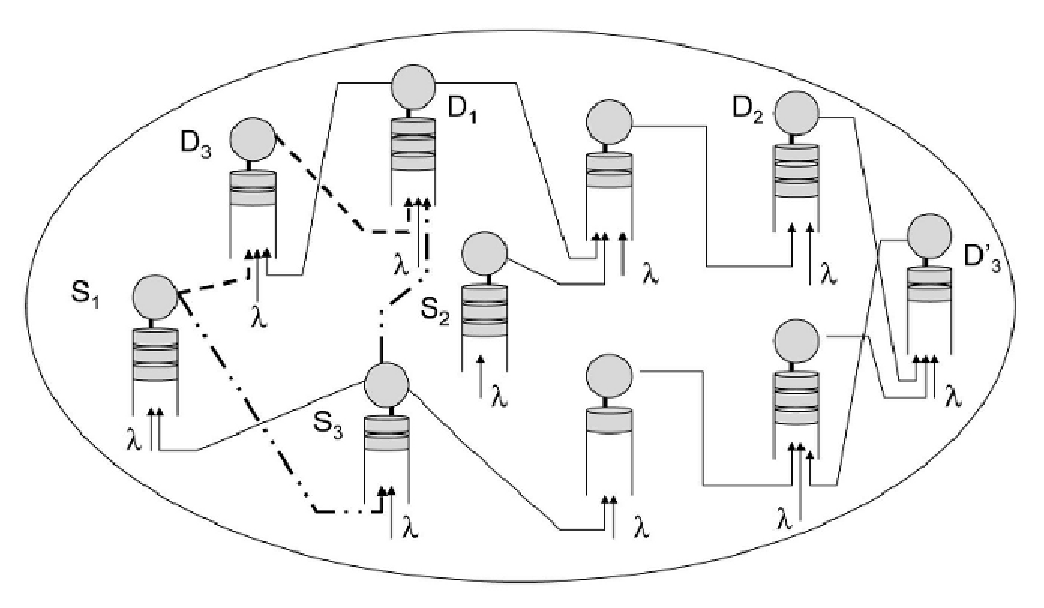
\includegraphics[scale=0.4]{./graph/nrb}
\caption{Bez rezervēšanas komutācijas modelis \cite{route_res}}
\label{fig:nrb}
\end{figure}

Kad $n_{a}$ mezgls saņem ziņojumu no $n_{b}$ mezgla ($n_{a}$ darbojas kā releja), $n_{a}$ ievieto saņemto ziņojumu bufera rindā kopā ar $n_{a}$ mezgla ģenerētiem ziņojumiem. Ziņojumi no šīs rindas tiek pārraidīti secīgi, saņemtiem un $n_{a}$ ģenerētiem ziņojumiem nav prioritātēs šajā rindā.
Šī ir \acs{NRBS} pamatatšķirība no \acs{RBS} komutācijas modeļa, kurā retranslējoši mezgli dod absolūtu prioritāti saņemtiem ziņojumiem un savu ziņojumu pārraidi pilnībā aptur. \ac{NRBS} modelī katrs daudzposma maršruts ir rindu tandēms un visu tīklu var uzskatīt kā rindu tandēmu (\figurename. ~\ref{fig:nrbTandem}).

\begin{figure}[htb!]
\centering
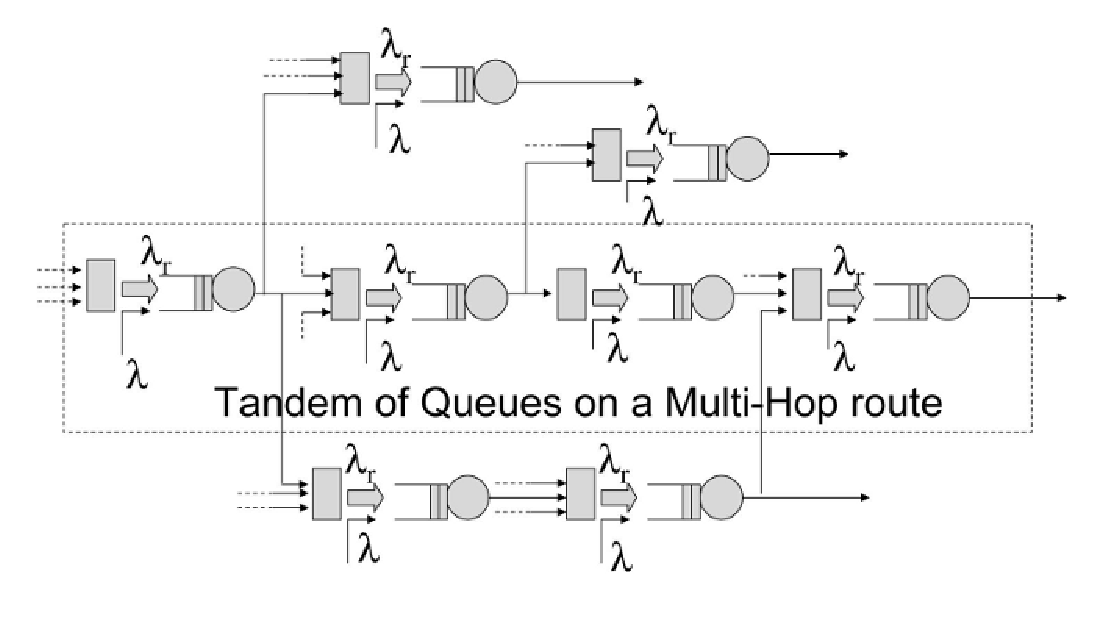
\includegraphics[scale=0.4]{./graph/tandem}
\caption{ Bez rezervēšanas komutācijas tandēmrinda \cite{route_res}}
\label{fig:nrbTandem}
\end{figure}

% \subsection{ Mobilitātes ietekme uz komutācijas modeļa veiktspēju}
% Pieņemsim, ka mobilie mezgli 1) pārvietojas ierobežota un konstanta pēc izmēra laukumā $A$ 2) vienmēr var atrast kaimiņ-mezglu uz $\Theta(1/\sqrt{\rho A})$ attālumā. Jāatzīmē ka, pastāv iespēja ka $\Theta(1/\sqrt{\rho A})$ attālumā kaimiņ-mezgls nav nekavējoties pieejams; tas izraisa pārraides aizkāvi no avota līdz galamērķim. Tīklā ar \ac{RBS} komutāciju savienojuma garums starp mobiliem mezgliem var paliecināties laikā un tas ietekmes tīkla robustumu. \ac{RBS} robustums ir daudzkārtēji mazināts ar mezglu mobilitāti salīdzinājumā ar \ac{NRBS}. Tīklā ar \ac{NRBS} komutāciju kad pārraide no avota ir sākusies  maršruta secīgas savienojuma izvēlēti  oportūnistiski, balstoties uz attāluma. Gadījuma ja divi noteikta maršruta secīgi mezgli pārāk attālinās viens no otra, savienojuma sakuma mezgls ( mezgls kas secīgi ir pirmais) izvēlas citu mezglu kas atrodas $\Theta(\sqrt{1/\rho A})$ attālumā. Lai nodrošināt šādu maršruta izveidi ir nepieciešama liela vadības ziņojumu (control message) apmaiņa starp retranslējošiem mezgliem.
